\documentclass[conference]{IEEEtran}
\IEEEoverridecommandlockouts
\usepackage{cite}
\usepackage{cancel}
\usepackage{amsmath,amssymb,amsfonts}
\usepackage{algorithmic}
\usepackage{siunitx}
\usepackage{graphicx}
\usepackage{float}
\usepackage{tikz}
\graphicspath{{images/}}
\usepackage{textcomp}
\def\BibTeX{{\rm B\kern-.05em{\sc i\kern-.025em b}\kern-.08em
    T\kern-.1667em\lower.7ex\hbox{E}\kern-.125emX}}
\begin{document}

\title{Segregating Robots That Do Not Compute}

\author{\IEEEauthorblockN{Jordan Burklund}
\IEEEauthorblockA{\textit{Worcester Polytechnic Institute} \\
Worcester, MA \\
jsburklund@wpi.edu}
\and
\IEEEauthorblockN{Michael Giancola}
\IEEEauthorblockA{\textit{Worcester Polytechnic Institute} \\
Worcester, MA \\
mjgiancola@wpi.edu}
\and
\IEEEauthorblockN{Peter Mitrano}
\IEEEauthorblockA{\textit{Worcester Polytechnic Institute} \\
Worcester, MA \\
pdmitrano@wpi.edu}
}

\maketitle

\begin{abstract}
  In this paper, we reproduce robot aggregation behavior from Gauci et al. \cite{gauci_self-organized_2014} on a swarm of Khepera IV robots. We then develop a fitness function to be used to evolve a controller for $n$-class robot segregation. Like \cite{gauci_self-organized_2014}, this solution will be computeless and memoryless.
\end{abstract}

\begin{IEEEkeywords}
  swarm robotics, robot aggregation, robot segregation
\end{IEEEkeywords}

\section{Introduction and Related Work}
  In our study of swarm robotics, we have read research on the clustering of robots and objects as a swarm.  Several of the methods proposed have demonstrated the ability to aggregate robots and objects in a distributed way, and some have shown the ability to perform such tasks with limited computation and sensing capabilities.

  Decentralized aggregation is frequently posed as a precursor to other swarm behaviors as \cite{gauci_evolving_2014} mentions. By aggregating, agents can cooperate on tasks, share information, and other higher level swarm behaviors.  In our work, we are investigating segregating agents into $n$ clusters, so that agents could perform some collective task within their own cluster.  This method will be decentralized and only rely on agents being able to sense one another such that environmental queues are not necessary.

  \subsection{Robot Aggregation}
    Robot aggregation is defined as having all robots in the swarm collect at a particular location in a distributed manner. Traditionally, swarm aggregation policies require compute bearing and distance to other robots, or to sense gradients in the environment, or otherwise communicate information. However, implementing these communication systems is difficult in practice, so methods that do not require communication or complex sensing are desirable. In \cite{gauci_self-organized_2014}, the authors propose a new class of policies that require no computation. In \cite{gauci_self-organized_2014,gauci_evolving_2014,kernbach_re-embodiment_2009,ando_distributed_1999}, the authors further make the distinction of memoryless policies, where the robot operates only on the current observed state (reactive), versus retaining information from previous states (recurrent).

    In \cite{ando_distributed_1999}, the authors present a robot aggregation model similar to \cite{gauci_self-organized_2014}. Their algorithm assumed that the robots have limited visibility, but allows the robots to perform computations to determine their next position. They prove that their algorithm is correct in theory, then run the algorithm in simulation. They evaluate the algorithm by measuring the total number of phases all robots execute and the total distance between each robot's starting position and their final position. They found that the location that the robots converged to wasn't significantly impacted by the degree of synchronization (i.e. how many robots move simultaneously), view obstruction, or sensor/control error.

    The work of \cite{gasparri_swarm_2012} does not restrict itself to a computeless or memoryless solution. Instead they develop an aggregation algorithm which enables robots to respond to guidance commands -- i.e., a human using hand gestures to indicate which direction the swarm should move. They show that swarms running their algorithm are able to follow guidance commands and stay aggregated without colliding.

  \subsection{Robots That Do Not Compute}

    Similar to \cite{gauci_self-organized_2014} and \cite{gauci_evolving_2014}, the authors of \cite{bahgeci_evolving_2005} propose an aggregation policy that executes only on current sensor information, and sensing capabilities are limited to local interactions. The robots in \cite{bahgeci_evolving_2005} have IR distance sensors surrounding the robot, 4 microphones, and an omni-directional speaker.  Rather than operating on a finite state of a single sensor as in \cite{gauci_self-organized_2014} and \cite{gauci_evolving_2014}, the policy is a linear combination of the IR sensor values and the intensity values of the microphones.  This emulates a single-layer neural network, where the outputs are the two wheel velocities and intensity of the speaker output.  The authors show that a genetic algorithm is able to find weights for the policy such that robots aggregate together.

    In \cite{kernbach_re-embodiment_2009}, the authors propose an aggregation policy roughly based on observations of bees clustering in an optimal temperature location. In their method, robots are only able to distinguish between collisions between another robot or a wall, can only sense the intensity of a light source when they have collided, and do not communicate information.  Although the robots have limited sensing and communication capabilities, the authors show that robots can aggregate to an optimal light intensity location, and that the time to converge to the optimal location improves with increasing number of robots in the environment.

    Robots that do not compute and are memoryless have also been shown to aggregate around a specific object, circle in a ring around an object, and forage for obstacles \cite{johnson_evolving_2016}. In this work, the authors show one can construct simple new fitness functions to guide the evolution of controllers to do new yet interesting tasks. However, they also report that in attempting to evolve a controller to rendezvous the robots around an object, they accidentally and consistently evolved a policy where the robots circled around the target object. This demonstrates that designing a fitness function can be hard or unreliable. They achieved rendezvous by initializing the policy at generation zero to the policy found in \cite{gauci_self-organized_2014} for simple aggregation. For our final project, this implies that although memoryless no-compute controllers are capable of interesting emergent behavior, it is not necessarily trivial to find the controller with the desired emergent behavior. At the very least, there is not a formal theory or robust algorithm for deriving these controllers for a specific behavior.

\section{Proposed Experiments and Expected Outcomes}

  Our first experiment will be to reproduce the work from \cite{gauci_self-organized_2014}. We want to demonstrate that the robots do in fact aggregate in a similar amount of time and with similar density as demonstrated by the original authors. We will evaluate the controller presented by \cite{gauci_self-organized_2014} for 10 trials with various starting distributions with ARGoS and Buzz on the Khepera IV. We are curious if there will be any difficulties or challenges in transferring from the e-puck platform used by the original authors. Additionally, we are interested in exploring the effect of starting distributions on the performance of the controller. In one set of tests, we will initialize the robots in several clusters spread throughout the arena. In another, we will put the robots in a single line.

  Our second experiment will be to evolve a controller for homogeneous aggregation, since the original authors used a grid-search method. This will also allow us to test our genetic algorithm and multi-threaded system. Again, we will evaluate the robot dispersion metric and convergence time for the various distributions described previously. To measure convergence time, we will use the number of time steps before the cluster reached 95\% of it's minimum dispersion.

  Our third experiment will be to extend aggregation to the case where the robots need to segregate into multiple classes. Robots are assigned to different classes based on their ID number, and we assume robots do not change their class during a trial. We will design a simple fitness function for $n$-class segregation. Our goal is for this function to be fast to compute and elegant. We will attempt to evolve a controller for $n$-class segregation, starting with just two classes and testing with an increasing number of distinct classes of robots. We hypothesize that the controllers will need to contain 6 parameters for three sensor states, building immediately upon the 4 parameters binary sensor controllers. The three states will be nothing, kin, and non-kin. We will again explore how various starting distributions effects the dispersion and convergence time. In addition to the distributions described above (i.e. clusters, single line) we will initialize the robots in a single, heterogeneous square lattice. For the cluster initialization, the clusters will be heterogeneous, so robots will have to navigate out of their current cluster to form a cluster of robots of the same type. Again, convergence time will be defined as the number of time steps before the cluster reached 95\% of minimum dispersion.

\section{Methodology}

  We first extended the binary sensor presented in \cite{gauci_self-organized_2014} to be able to detect multiple types of robots. We again use the range and bearing sensor, this time with simulated FootBots, to detect whether a robot is in line of sight. If there is no robot, the sensor returns 0 like in \cite{gauci_self-organized_2014}. If there is a robot, then the sensor returns 1 if the robot is kin (in the same class), or non-kin (in any other class).

  In order to avoid manually spending time picking parameters or spending tremendous compute time using grid-search time find parameters, we use a simple genetic algorithm to evolve controller parameters. In all our experiments, we use 6 parameters for nothing, kin and non-kin, where each parameter ranges from -1 to 1. In our controller, we then scale this parameter to range from -20cm/s to 20cm/s. We treat aggregation as a special case of 1 class segregation, in which case the final two parameters of the controller are never used. The genetic algorithm we used is unmodified from the example MPGA code provided with the ARGoS simulator. The mutation strategy is simply to mutate each of these 6 parameters with some probability p ($0.05$ in our experiments). If a parameter is selected to be mutated, a uniformly random number from -1 to 1 is picked for the new value. Selection is performed by picking the two most fit individuals (the ones with lowest cost in our formulation), and then forming the next population by crossing the parameters of these two individuals. The original two parents are always kept in the population so that the current fittest individual is never removed until a more fit genome is discovered.

  As with any genetic algorithm, it is important to have a fitness function that accurately assigns cost to behaviors. In this project, we plan to explore three different cost functions. The first is the cluster metric used by \cite{gauci_self-organized_2014}, which is the proportion of the number of robots in the largest cluster to the total number of robots. we will apply this for each class of robots and sum up the cost for each class to get the total cost. Further, we will determine the percentage of trials that reach one cluster per class by then end of some number of time steps.

  We also propose two new cluster metrics to use as fitness functions. The cluster metric described above is problematic because it considers a straight line of robots to be one cluster. In some scenarios, we care about how tightly the swarm is packed in its clusters. Consider the scenario where different classes of swarm robots needs to be collected after a mission, and the must be sorted into clusters so that they can be air-lifted easily. With this secnario im mind, we propose a new metric which uses the convex hull of the robots in each class. We want to penalize a large convex hull, so the first time is simply the area of the convex hull. The second term assigns cost to the presence of non-kin inside the convex hull. Computing the convex hull can be done with Garaham's Scan algorithm, and computing the area is the sum the cross products around each vertex.

  $$ c_{\text{pack}} = A_\text{convex hull} + \frac{\text{number of non-kin robots inside convex hull}}{\text{number of non-kin robots}}$$

  The final fitness function we will test attempts to minimize intra-class dispersion while also maximize inter-class dispersion. We borrow the dispersion metric $u^{(t)}$ from \cite{gauci_self-organized_2014}, which essentially computes the sum of distances from each robot to the centroid. Consider $u_i^{(t)}$ to be the dispersion of a particular class $i$ at time $t$. Given all the centroids $\bar{p}_i^{(t)}$ for each class $i$, we call the centroid of all of these centroids $\bar{P}^{(t)}$. Our overall cost (which is the negative of fitness) is defined as follows:

  \begin{align*}
  c_{\text{intra}} &= \sum_{i=1}^n u_i^{(t)} \\
  c_{\text{inter}} &= -\frac{1} {4r^2}\sum_{i=1}^n{\lVert \bar{p}_i^{(t)} - \bar{P}_i^{(t)} \rVert}^2 \\
  c_{\text{total}} &=  \sum_{t=0}^{T-1} t (c_{\text{intra}} + c_{\text{intra}}) \\
  \end{align*}


  \subsection{What Didn't Work}

  When we implemented the centroid-of-centroids style cost function, we quickly found examples of configurations ranked in ways we did not like. One example is shown below in Figure \ref{fig:cost_function_fuckup}. The behavior that looks like aggregation was given lower cost of -8e9, versus the behavior that looks like segregation was given a cost of -5e9.

  \begin{figure}
    \centering
    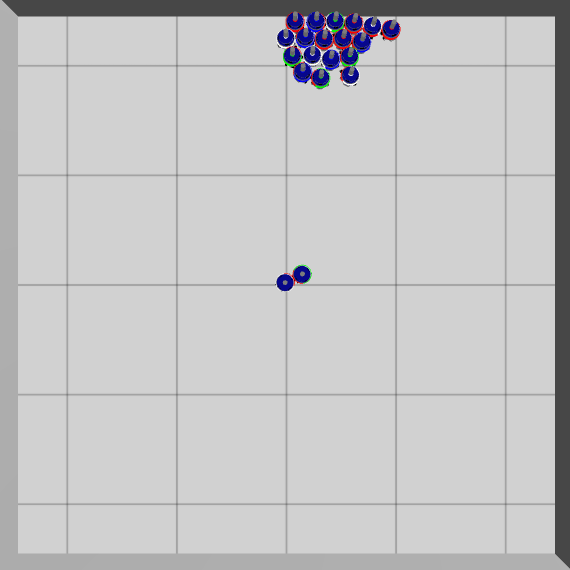
\includegraphics[width=0.49\linewidth]{./images/individual_0_gen_0.png}
    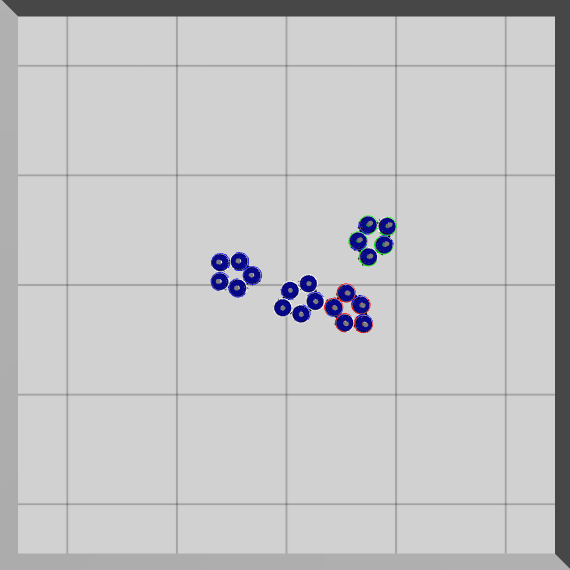
\includegraphics[width=0.49\linewidth]{./images/individual_0_gen_1_better.png}
    \caption{The left picture was given lower cost than the right, which is not desirable.}
    \label{fig:cost_function_fuckup}
  \end{figure}



\section{Controller Analysis}

  We found imperically that the parameters [0.5 -0.5 -0.2 0.6 0.6 0.2] successfully acheive segregatation. We now analyze this controller formally. First, we prove that a single isolated robot executing this controller will aggregate to a kin robot, or more importantly, a cluster of kin robots. This proof is an extension of the Theorem 5.1 provided in \cite{gauci_self-organized_2014}. Consider a robot situated as shown in Figure \ref{fig:kin_aggregation}. The controller dictates that since a Kin robot is seen, $I=1$, so $v_{l_1} = -0.2$ and $v_{r_1} = 0.6$. This will cause the robot to turn with some radius $R$. Without loss of generality, we define our coordinate system so that $c_i=[0,0]$ with the robot facing the $+x$ axis. For this analysis, we assume that the robot has a fixed, positive inter wheel distnace $W$, and that the controller is executed in small finite time steps. Our goal is to show that the distance between the positon of the robot after executing our controller for one time step $p'_i$ and the kin robot $p_j$ is less than the distance between the initial position of the robot $p_i$ and the kin robot $p_j$. Formally, this is expressed by the following relationship:

  \begin{figure}[H]
    \centering
    \begin{tikzpicture}
      \draw[->] (0,0) -- (7,0);
      \node at (7.2,.2) {x};
      \draw[->] (0,0) -- (0,3);
      \node at (-0.2,3.2) {y};

       % c_i
      \filldraw (0,0) circle (.05);
      \node at (.2,.2) {$c_i$};
      \draw[blue, dashed] (0,0) circle (2);

       % p_i
      \filldraw (0,-2) circle (.05);
      \node at (.2,-2.2) {$p_i$};
      \draw[blue] (0,-2) circle (0.85);
      \node at (-.3,-.8) {$R$};
      \draw[dashed] (0,0) -- (0,-2);

       % p'_i
      \filldraw (1.41,-1.41) circle (.05);
      \node at (1.85,-1.25) {$p'_i$};
      \draw[blue] (1.41,-1.41) circle (0.85);
      \draw[dashed] (0,0) -- (1.41,-1.41);
      \node at (.8,-.3) {$R$};

       % p_j
      \filldraw (5,-3.25) circle (.05);
      \node at (5.2,-3.5) {$p_j$};
      \draw[red] (5,-3.25) circle (1.25);
      \draw (5,-3.25) -- (5,-2);
      \node at (5.3,-2.625) {$r_j$};

      % delta
      \draw[blue] (0,-2) -- (5,-2);
      \draw[blue] (1.41,-1.41) -- (5.3,-2.03);
      \node at (2.5, -2.2) {$\delta$};

      % theta
      \draw (0,-.7) arc [radius=.7, start angle=-90, end angle=-45];
      \node at (.36,-.85) {$\theta$};
    \end{tikzpicture}
    \caption{The robot will always move closer to its Kin.}
    \label{fig:kin_aggregation}
  \end{figure}

  \begin{equation} \label{eq:agg}
    \lVert p_j - p'_i \rVert < \lVert p_j - p_i \rVert
  \end{equation}

  We emphisize that $r_j$ could be the radius of a single kin robot or the radius of a large cluster of kin robots. With this coordinate system and assumptions stated, we can define the coordinate of $p_i$, $p_j$, and $p'_i$.

  \begin{equation}
    \begin{split}
      p_i = \begin{bmatrix}0 \\ -R\end{bmatrix} \\
      p_j = \begin{bmatrix}\delta \\ -(R+r_j)\end{bmatrix} \\
      p'_i = \begin{bmatrix}R\sin(\theta) \\ -R\cos(\theta)\end{bmatrix}
    \end{split}
  \end{equation}

  We then substitute these variables into our inequality (Equation \ref{eq:agg}), and the result is shown in Equation \ref{eq:agg_result}. For the full derivation, see Appendix \ref{thm:1}. In short, the distance of the robot to its kin is guaranteed to decrease until a point where the sensor ray distance $\delta$ is not greater than some simple function of $\theta$ and $R$. The dependant variables $\theta$ and $R$ are themselves a function of the inter wheel diameter $W$ and the wheels speeds of the controller $v_{l_1}$ and $v_{l_1}$, which are shown in Equation \ref{eq:theta_and_r}.

  \begin{equation} \label{eq:agg_result}
    \delta > (R + r_j)\tan\bigg(\frac{\theta}{2}\bigg)
  \end{equation}

  \begin{align}
    \begin{split} \label{eq:theta_and_r}
      \theta &= \Delta t\omega = \Delta t \frac{v_{r_1} - v_{l_1}}{W} = \Delta t \frac{0.6 - (-0.2)}{W} = \frac{0.8\Delta t}{W} \\
      R &= \frac{W}{2}\bigg(\frac{v_{r_1} + v_{l_1}}{v_{r_1} - v_{l_1}}\bigg) = \frac{W}{2}\bigg(\frac{0.6 + (-0.2)}{0.6 - (-0.2)}\bigg) = \frac{W}{4}
    \end{split}
  \end{align}

  Combining \ref{eq:theta_and_r} with \ref{eq:agg_result}, we get a useful expression that tells us the conditions under which aggregation is guaranteed. We emphasize that this does not mean aggregation to a kin is guaranteed for all values of $\Delta t$, $r_j$, and $W$. For example, if $\Delta t$ is increased to \SI{1}{\second} then aggregation is likely not guaranteed.

  \begin{equation*} \label{eq:agg_final_result}
    \delta > \bigg(\frac{W}{4} + r_j\bigg)\tan\bigg(\frac{0.8\Delta t}{2W}\bigg)
  \end{equation*}

  We can now consider an example with the Khephera IV robot, which we used in all our simulation. The inner wheel distance for the Khephera IV is \SI{0.14}{\meter}, and in our simulations we use a time step of $\Delta t = 0.1s$. Therefore $\theta = 0.5714\;\text{rad}$, and so aggregation is guaranteed when the following is true.

  \begin{equation} \label{eq:khephera_agg}
    \begin{split}
      \delta &> \bigg(0.035 + r_j\bigg)\tan\frac{0.5714}{2*0.14} \\
      \delta &> -1.96904 r_j - 0.06892
    \end{split}
  \end{equation}

   Note the largest possible value on the right hand side is achieved when $r_j=0$, at which point it equals $-0.06892$. However, since the distance between two robots $\delta$ must always be positive it will always be greater than $-0.06892$, we can say that it is guaranteed that Equation \ref{eq:khephera_agg} holds true for any $r_j$.

\section{Results}

  \subsection{Evaluating The Gauci Parameters on Khephera IV}

  So far, we have completed our first proposed work of applying the aggregation parameters from \cite{gauci_self-organized_2014} to a simulation with the Khephera IV robot. We implemented the controller using Buzz. Our ``binary sensor'' was simulated by checking if any robots were within 15 degrees of line of sight according to the range and bearing sensors. We ran 10 trials with 10 robots each and plotted the dispersion metric used by the original authors over time below in Figure \ref{fig:dispersion_gauci}. The green line show the dispersion cost for an optimal packing (7.47). Over the 10 trials, the lowest dispersion we found was 19.06, which is close to the optimal packing. This illustrates that the policy reported in \cite{gauci_self-organized_2014} is effective on the Khephera IV, which most notably is a different size, with no modifications. However, it does not quite achieve as close to the optimal packing as the authors report for the e-puck using the same parameters.

  \begin{figure}
    \centering
    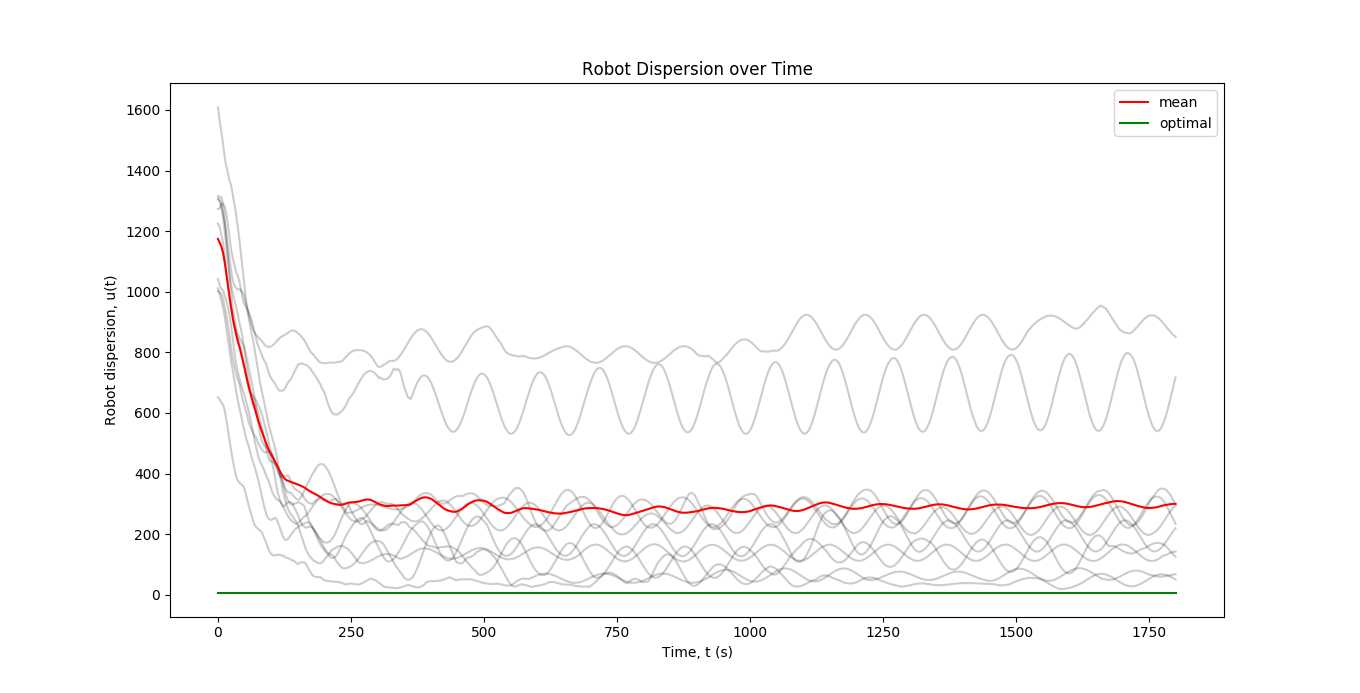
\includegraphics[width=1\linewidth]{./images/robot_dispersion_over_10_trials.png}
    \caption{The dispersion metric over time for 10 trials in simulation.}
    \label{fig:dispersion_gauci}
  \end{figure}

  \subsection{Evolving Aggregation}

  We have also successfully evolved no-compute one-class segregation, or simple aggregation policies. We have so far implemented only the third cluster cost function, but we have successfully used it to evolve aggregation. We show an example of this below. In this example, the cost (higher is less fit) of the bad individual had an average of 9.8659e+08 over 10 trials. The best individual in the second generation had an average cost of 1.0434e+07. This along with visual inspection shows our cost function and genetic algorithm are working.

  \begin{figure}
    \centering
    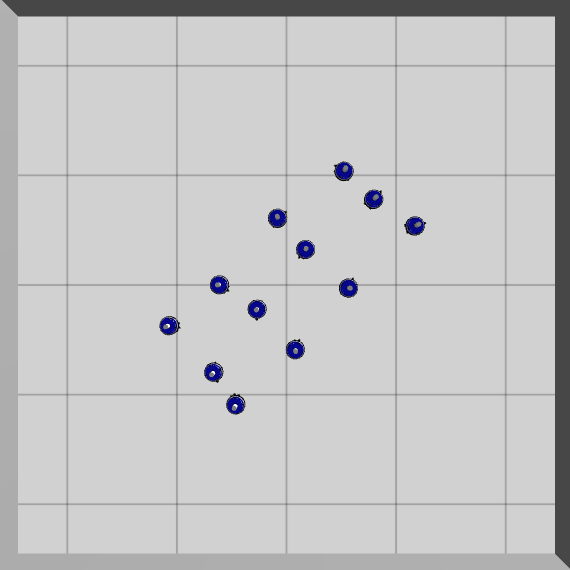
\includegraphics[width=0.49\linewidth]{./images/0_steps.png}
    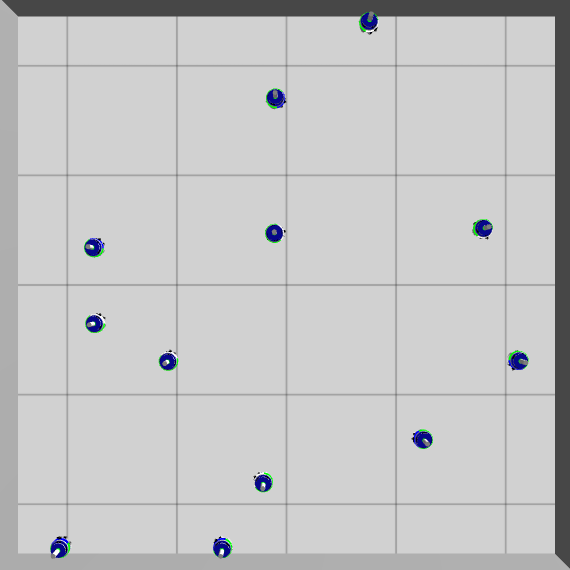
\includegraphics[width=0.49\linewidth]{./images/500_steps_individual_4_generation_0.png}
    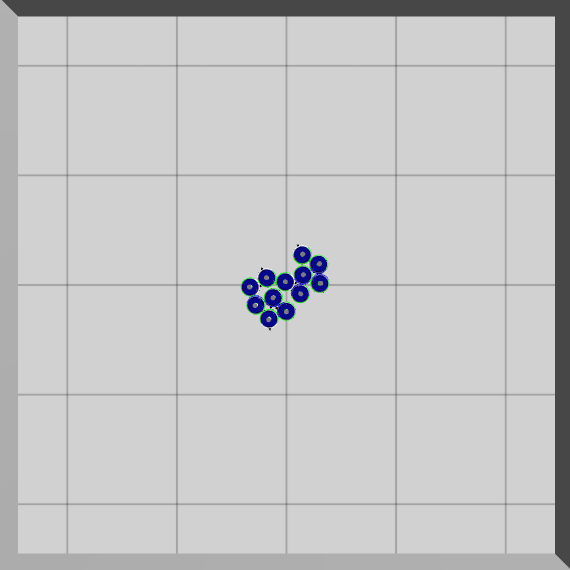
\includegraphics[width=0.49\linewidth]{./images/500_steps_individual_0_generation_2.png}
    \caption{The top left plot show the initial configuration. The top right plot shows the worst individual in the first generation, and the bottom shows the best individual in the second generation. Both are shown at 500 time steps.}
    \label{fig:evolved_aggregation}
  \end{figure}

  \subsection{Evolving $N$-Class Segregation}

  We also have started testing no-compute segregation policies and have found promising results so far. For simple validation, we searched by hand for segregation policies were able to easily find several policies for segregation. The hand selected policy that we experimented with appears to generalize across $n$ classes of robots. However, the policies do not seem to be as robust to various starting configurations or work very well if different numbers of robots. In figures \ref{fig:handtuned-2class}, \ref{fig:handtuned-3class}, and \ref{fig:handtuned-5class}, a hand selected policy is applied to the segregation task with differing numbers of classes. In these initial experiments, the same policy was used for all 3 experiments. This demonstrates that a genetic algorithm should be able to find a policy that segregates robots by classes as long as the fitness measure is able to assign cost behaviors correctly.

  \begin{figure}
    \centering
    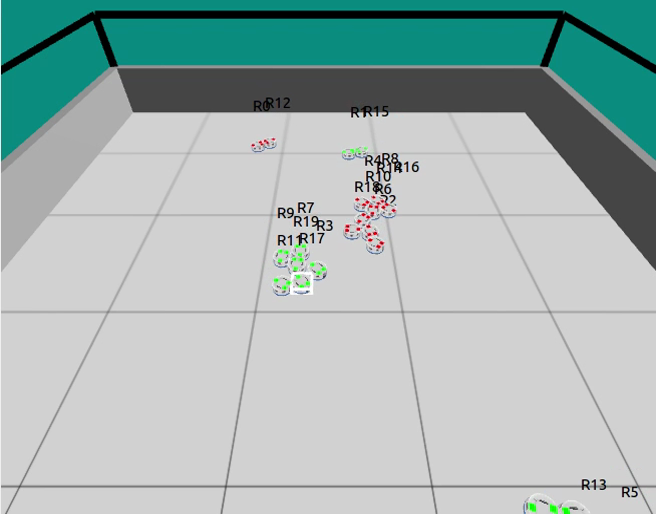
\includegraphics[width=8cm]{handtuned-2class.png}
    \caption{2 class Segregation with Hand Selected Policy}
    \label{fig:handtuned-2class}
  \end{figure}

  \begin{figure}
    \centering
    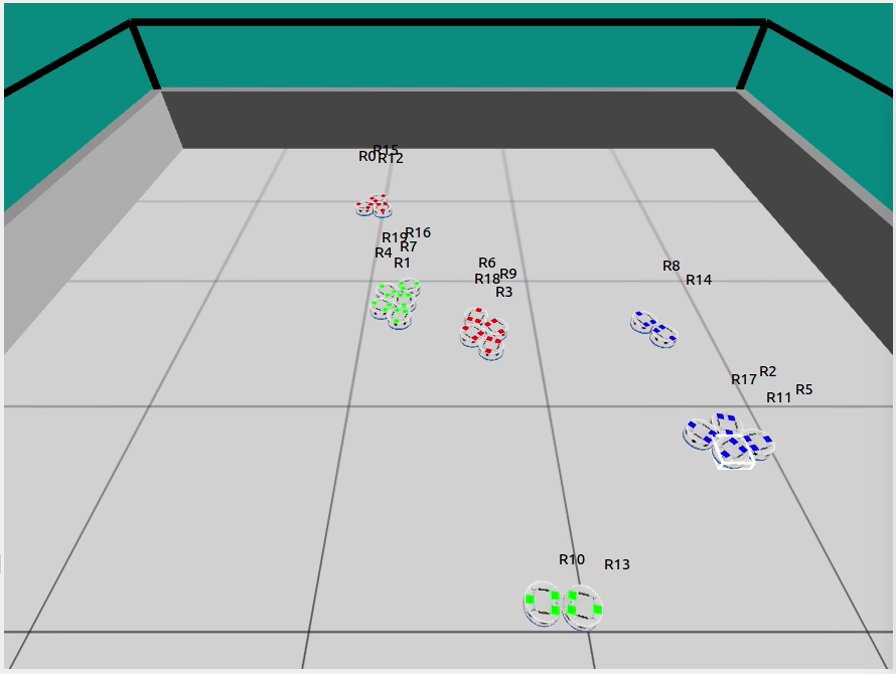
\includegraphics[width=8cm]{handtuned-3class.png}
    \caption{3 class Segregation with Hand Selected Policy}
    \label{fig:handtuned-3class}
  \end{figure}

  \begin{figure}
    \centering
    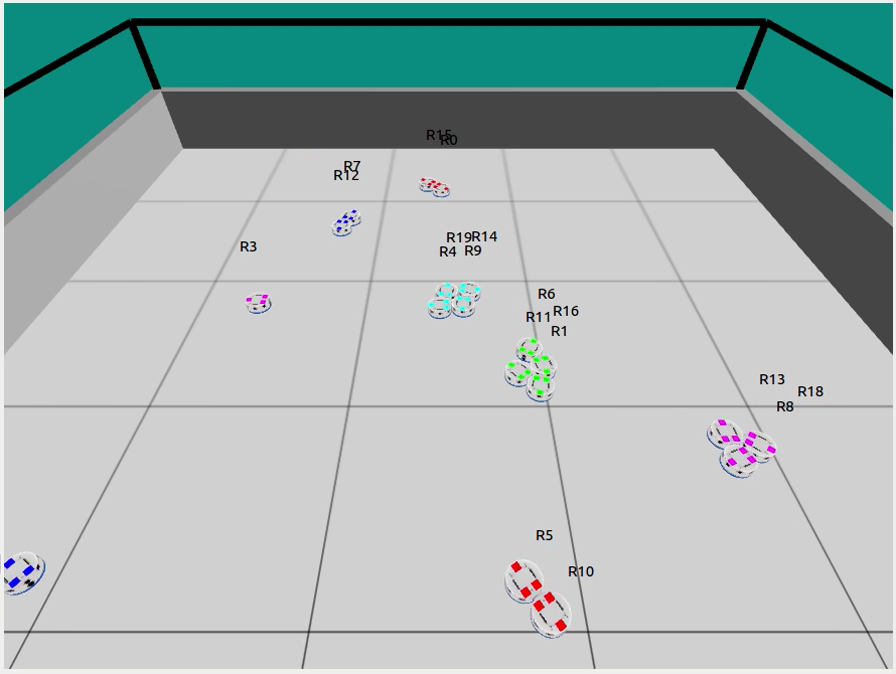
\includegraphics[width=8cm]{handtuned-5class.png}
    \caption{5 class Segregation with Hand Selected Policy}
    \label{fig:handtuned-5class}
  \end{figure}

In addition to the hand-selected policy, we have also started testing with our genetic algorithm to find a policy that segregates robots of multiple classes.  We implemented the third cost function in an attempt to evolve a behavior similar to the hand-selected policy.  The genetic algorithm is able to evolve a behavior, but we aren't yet getting the desired results.  For the genetic algorithm evaluated on 10 generations with several classes of robots, there appears to be a sort of circling behavior where robots of one class follow robots of another (fig. \ref{fig:ga-multiclass}).

  \begin{figure}
    \centering
    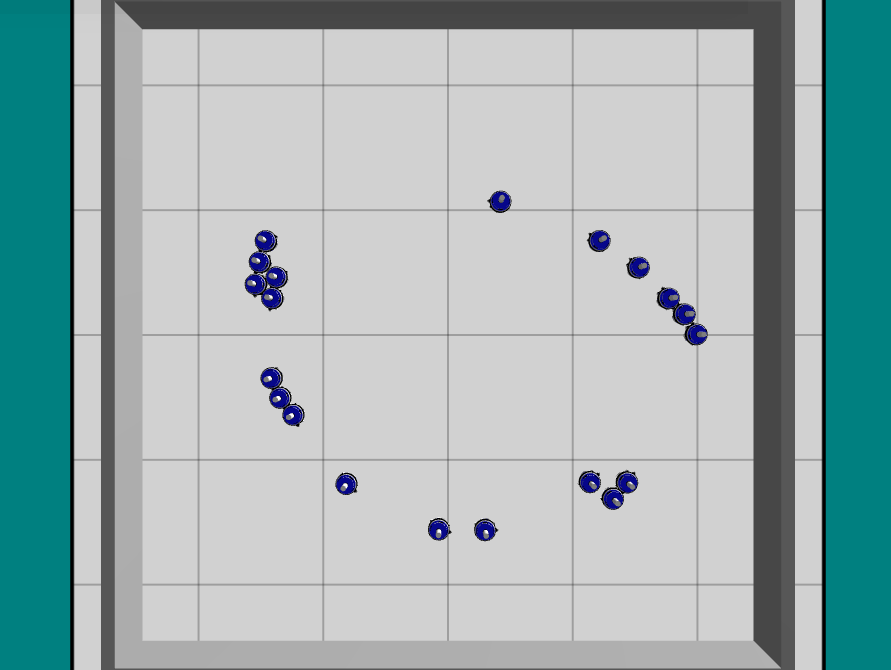
\includegraphics[width=8cm]{evolved_multiclass.png}
    \caption{Genetic Algorithm Evolved Behavior}
    \label{fig:ga-multiclass}
  \end{figure}

\section{Future Work}
%  - consider the radius of the robot, track width, etc...


\bibliography{RBE595.bib}
\bibliographystyle{unsrt}

\onecolumn
\section{Appendix}

\subsection{Proof of Theorem 1} \label{thm:1}

    \begin{align*}
      \lVert p_j - p'_i \rVert &< \lVert p_j - p_i \rVert \\
      \sqrt{(p_{j_x} - p'_{i_x})^2 + (p_{j_y} - p'_{i_y})^2} &< \sqrt{(p_{j_x} - p_{i_x})^2 + (p_{j_y} - p_{i_y})^2} \\
      (p_{j_x} - p'_{i_x})^2 + (p_{j_y} - p'_{i_y})^2 &< (p_{j_x} - p_{i_x})^2 + (p_{j_y} - p_{i_y})^2 \\
      (\delta - R\sin(\theta))^2 + (-(R+r_j) + R\cos(\theta))^2 &< \delta^2 + (-(R+r_j) + R)^2 \\
      (\delta - R\sin(\theta))^2 + (-(R+r_j) + R\cos(\theta))^2 &< \delta^2 + r_j^2 \\
      \delta^2 - 2R\delta\sin(\theta) + R^2\sin(\theta)^2 + (r_j + R(1 - \cos(\theta))^2 &< \delta^2 + r_j^2 \\
      \delta^2 - 2R\delta\sin(\theta) + R^2\sin(\theta)^2 + r_j^2 + 2Rr_j(1 - \cos(\theta)) + R^2(1 - \cos(\theta))^2 &< \delta^2 + r_j^2 \\
      \delta^2 - 2R\delta\sin(\theta) + R^2\sin(\theta)^2 + r_j^2 + 2Rr_j - 2Rr_j\cos(\theta) + R^2(1 - \cos(\theta))^2 &< \delta^2 + r_j^2 \\
      \delta^2 - 2R\delta\sin(\theta) + R^2\sin(\theta)^2 + r_j^2 + 2Rr_j - 2Rr_j\cos(\theta) + R^2(1 - 2\cos(\theta) + \cos(\theta)^2) &< \delta^2 + r_j^2 \\
      \delta^2 - 2R\delta\sin(\theta) + R^2\sin(\theta)^2 + r_j^2 + 2Rr_j - 2Rr_j\cos(\theta) + R^2 - 2R^2\cos(\theta) + R^2\cos(\theta)^2 &< \delta^2 + r_j^2 \\
      \delta^2 - 2R\delta\sin(\theta) + R^2(\sin(\theta)^2 + cos(\theta)^2) + r_j^2 + 2Rr_j - 2Rr_j\cos(\theta) + R^2 - 2R^2\cos(\theta) &< \delta^2 + r_j^2 \\
      \cancel{\delta^2} - 2R\delta\sin(\theta) + 2R^2 + \cancel{r_j^2} + 2Rr_j - 2Rr_j\cos(\theta) - 2R^2\cos(\theta) &< \cancel{\delta^2} + \cancel{r_j^2} \\
      -2R\delta\sin(\theta) + 2R^2 + 2Rr_j - 2Rr_j\cos(\theta) - 2R^2\cos(\theta) &< 0 \\
      -\delta\sin(\theta) + R + r_j - r_j\cos(\theta) - R\cos(\theta) &< 0 \qquad \text{assuming $R>0$}\\
      R + r_j - r_j\cos(\theta) - R\cos(\theta) &< \delta\sin(\theta) \\
      r_j(1 - \cos(\theta)) + R(1 - \cos(\theta)) &< \delta\sin(\theta) \\
      (r_j+R)(1 - \cos(\theta)) &< \delta\sin(\theta) \\
      (R+r_j)\bigg(\frac{1 - \cos(\theta)}{\sin(\theta)}\bigg) &< \delta \\
      (R+r_j)\tan{\frac{\theta}{2}}  &< \delta \\
    \end{align*}

\end{document}
